\chapter{Изработка на работоспособен модел}
\indent{}
Разработването на системата започна с проучване на РОБКО 01 и въстановяване на принципната му схема. Проектирането на основната платка и PATA адаптера протече успоредно с работата по софтуера. Преди завършването на основната платка за връзка между робота и микроконтролера се използваше тестовия адаптер, показан на фигура \ref{fig:test_adapter}.\\
\begin{figure}[!h]
    \centering
    \begin{subfigure}{0.48\textwidth}
        \centering
        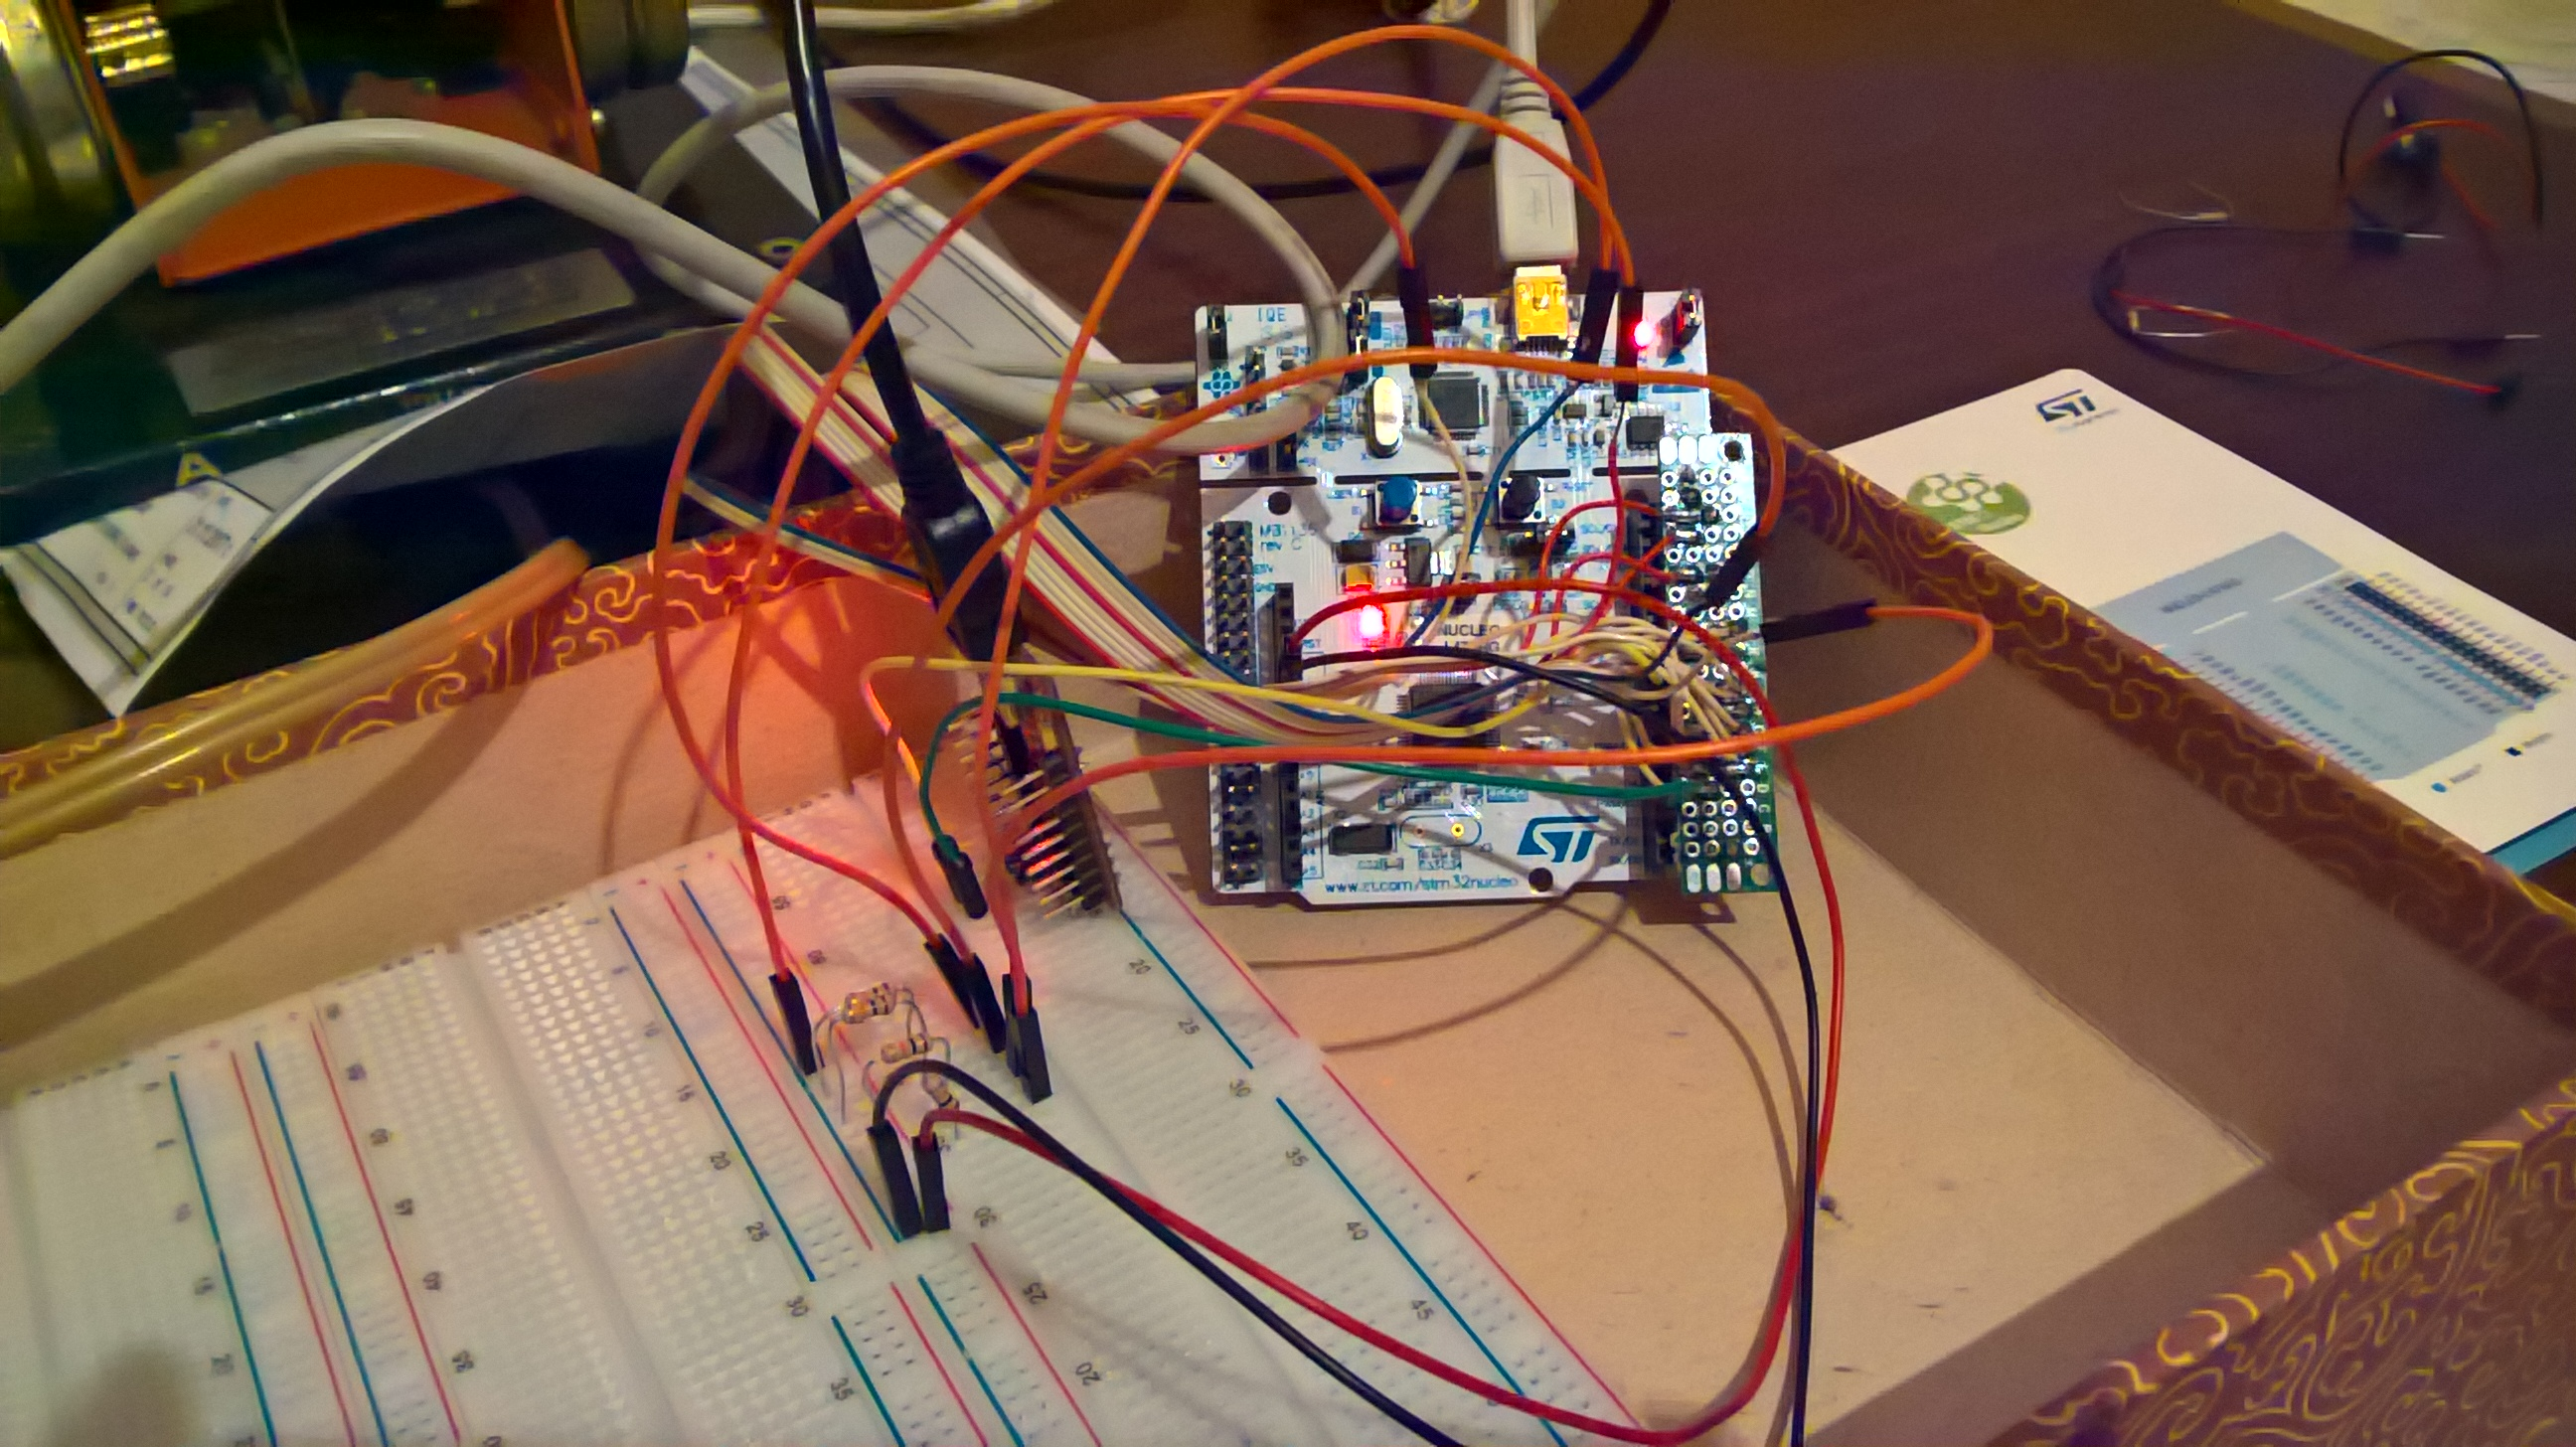
\includegraphics[width=\linewidth]{pictures/test_adapter_1.jpg}
    \end{subfigure}
    \hfill%
    \begin{subfigure}{0.48\textwidth}
        \centering
        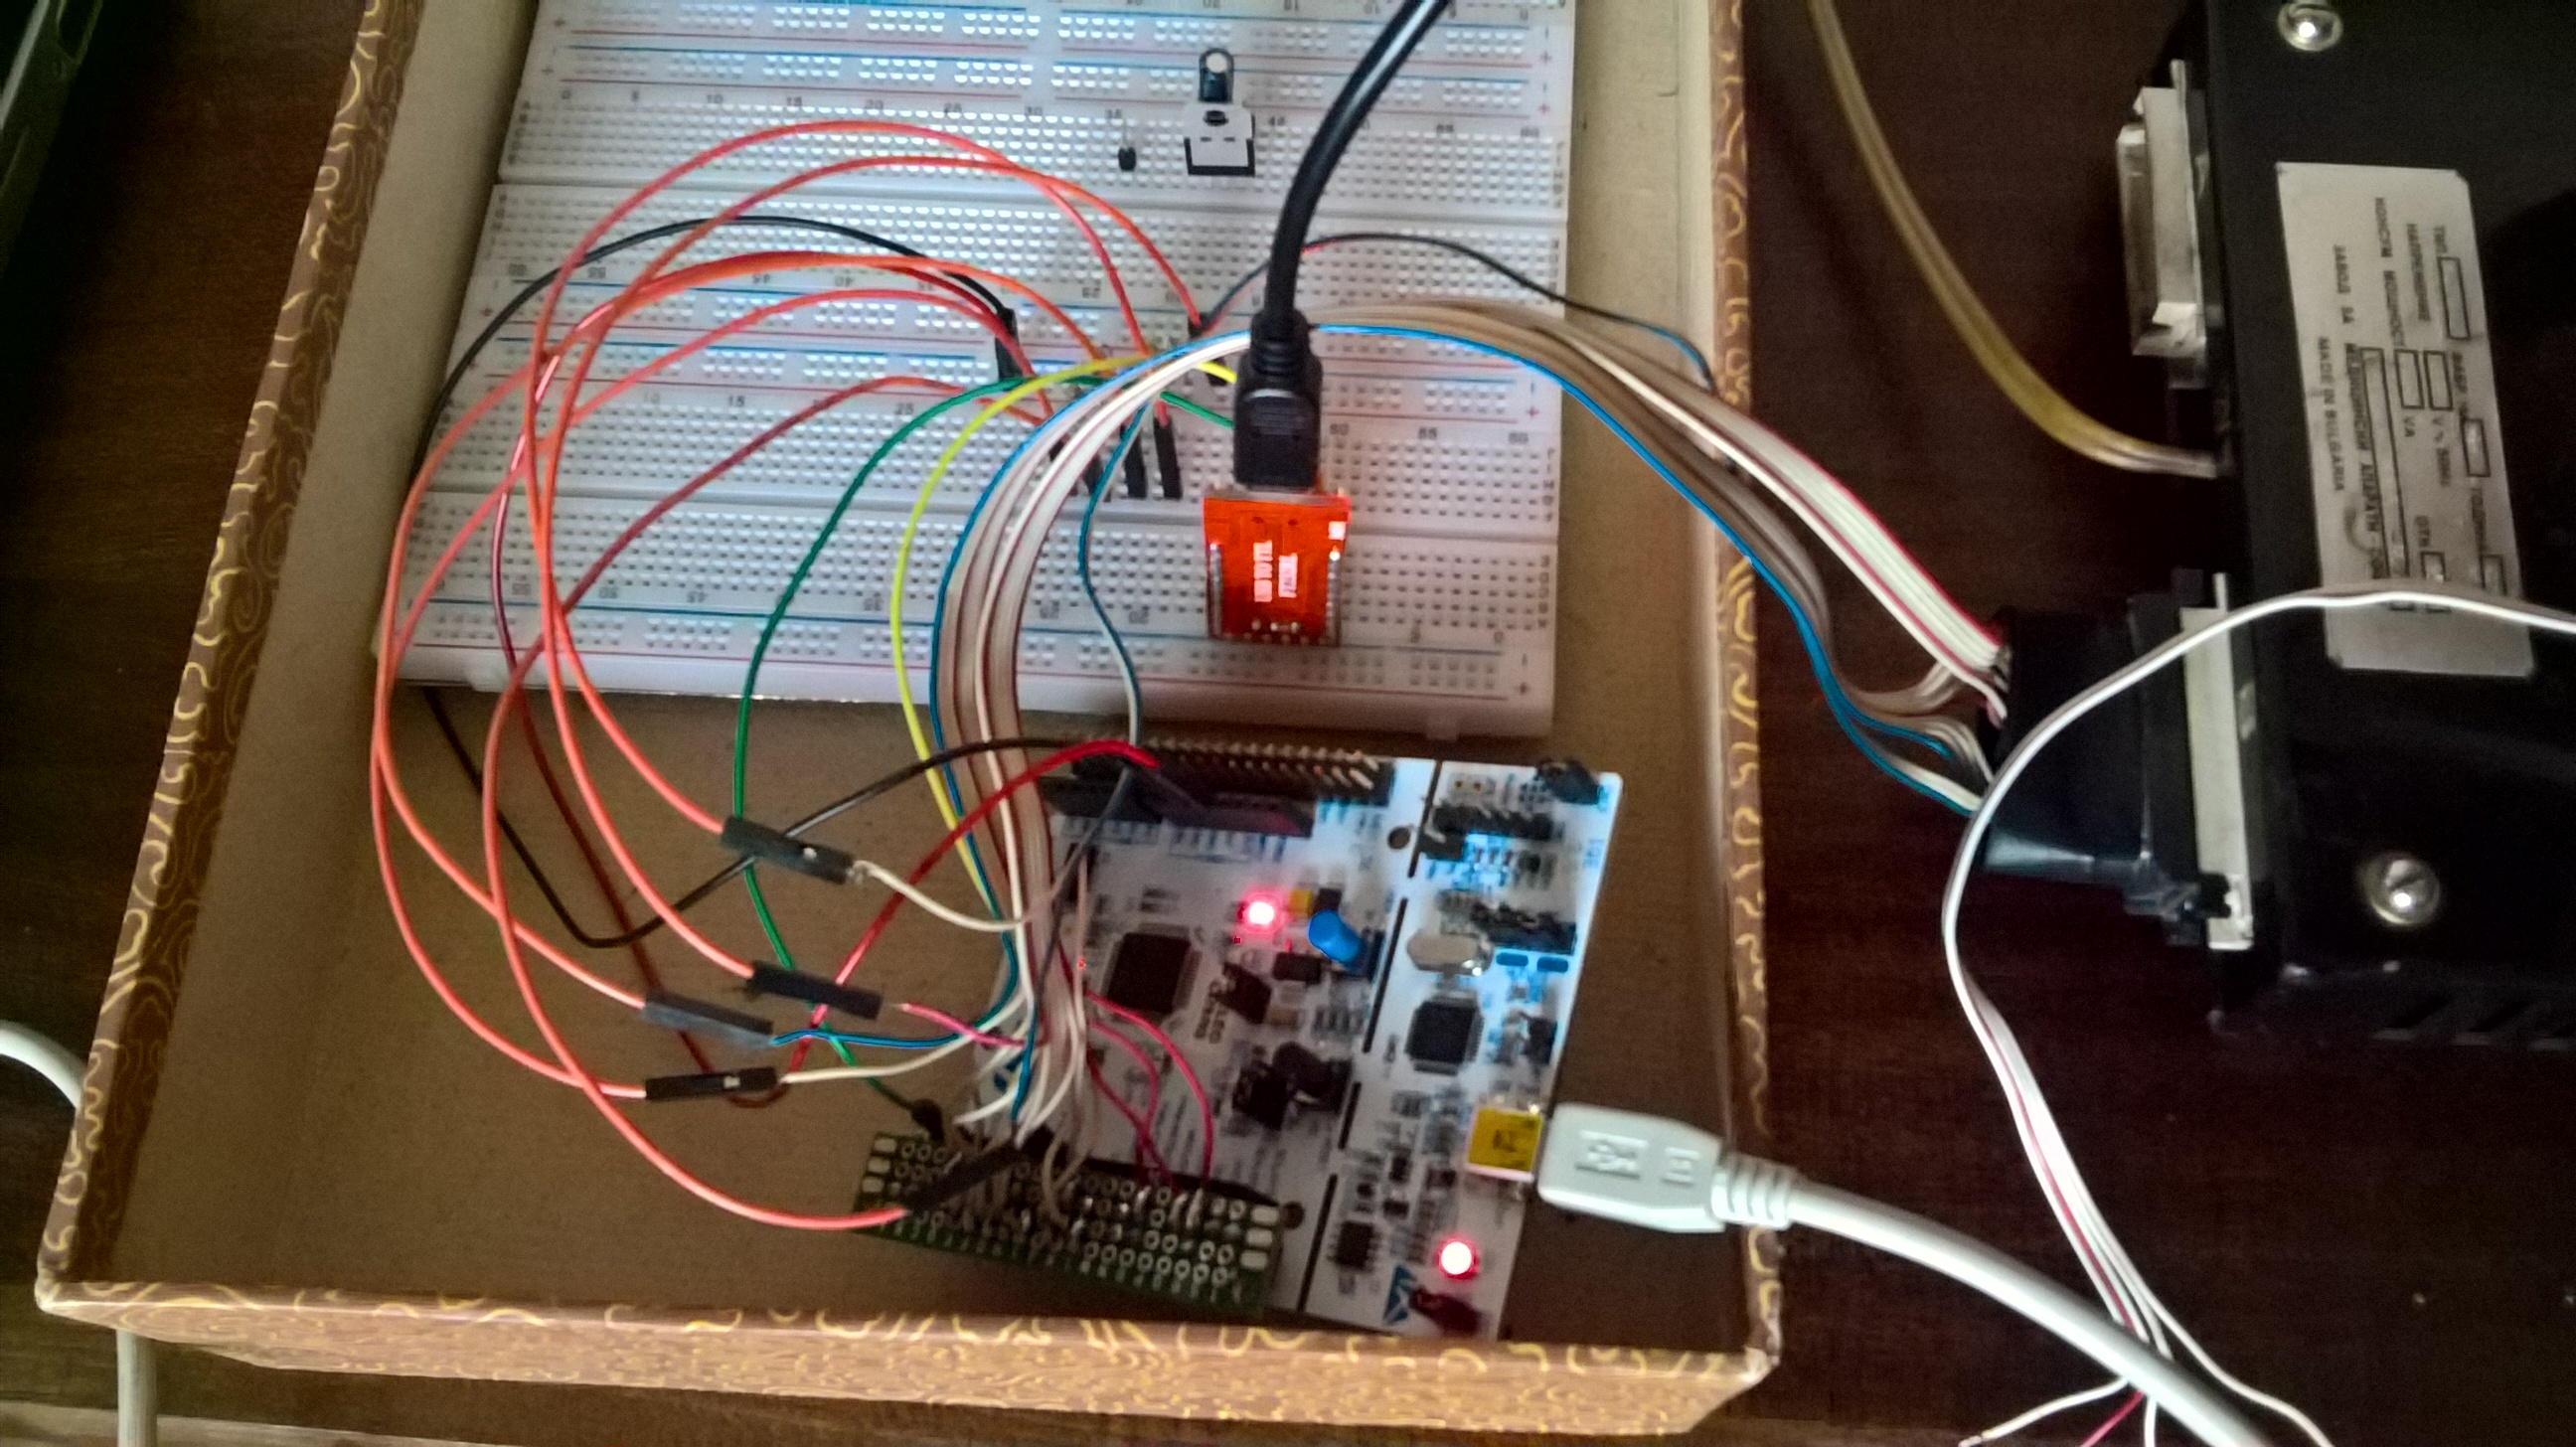
\includegraphics[width=\linewidth]{pictures/test_adapter_2.jpg}
    \end{subfigure}
    \caption{Тестов адаптер и микроконтролерна платка}
    \label{fig:test_adapter}
\end{figure}
\indent{}
Основната платка е проектирана на CAD програмата Proteus 8, която изгражда триизмерен модел на печатните платки (фиг. \ref{fig:3D}). Прототипът на основната платка (фиг. \ref{fig:main_board_proto}) е произведен с помощта на CNC фреза в София Тех Парк. Чрез него бяха открити някои неточности в проектираната печатна платка. След коригиране на грешките беше произведен по класическа технология втори вариант на платката (фиг. \ref{fig:main_board_real}).\\
\begin{figure}[!h]
    \centering
        \begin{subfigure}{0.32\textwidth}
        \centering
        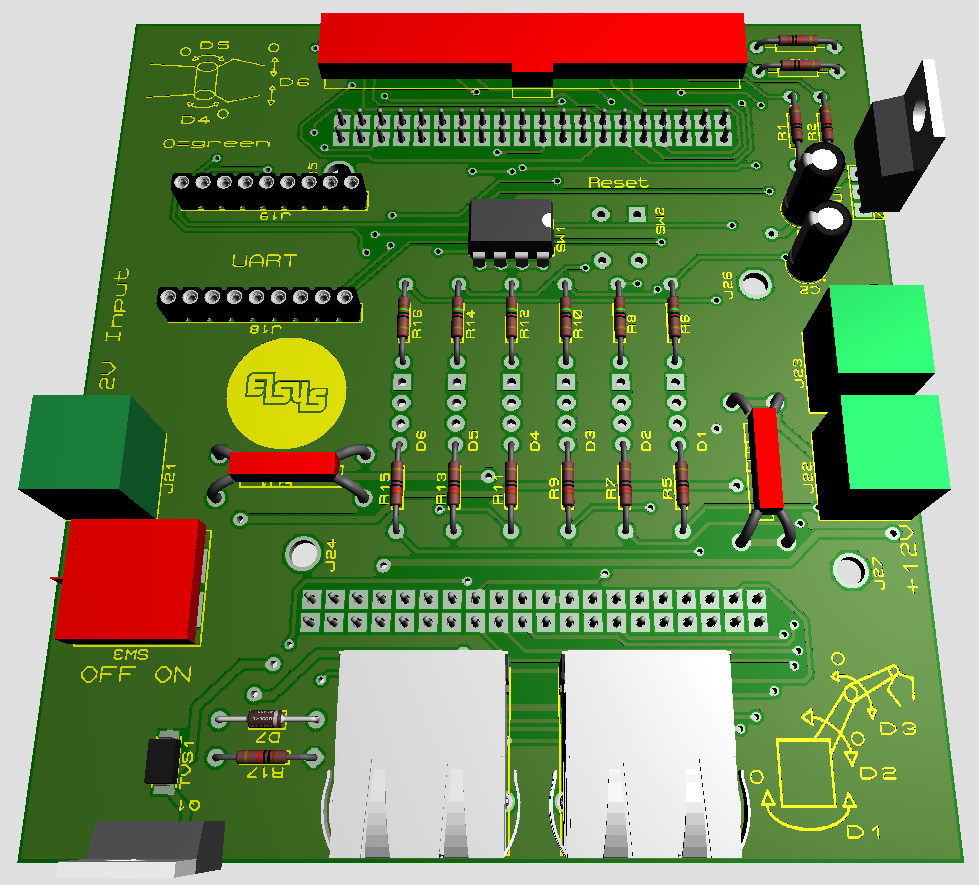
\includegraphics[width=\linewidth]{pictures/3D_view.PNG}
        \caption{Триизмерен модел}
        \label{fig:3D}
    \end{subfigure}
    \hfill%
    \begin{subfigure}{0.32\textwidth}
        \centering
        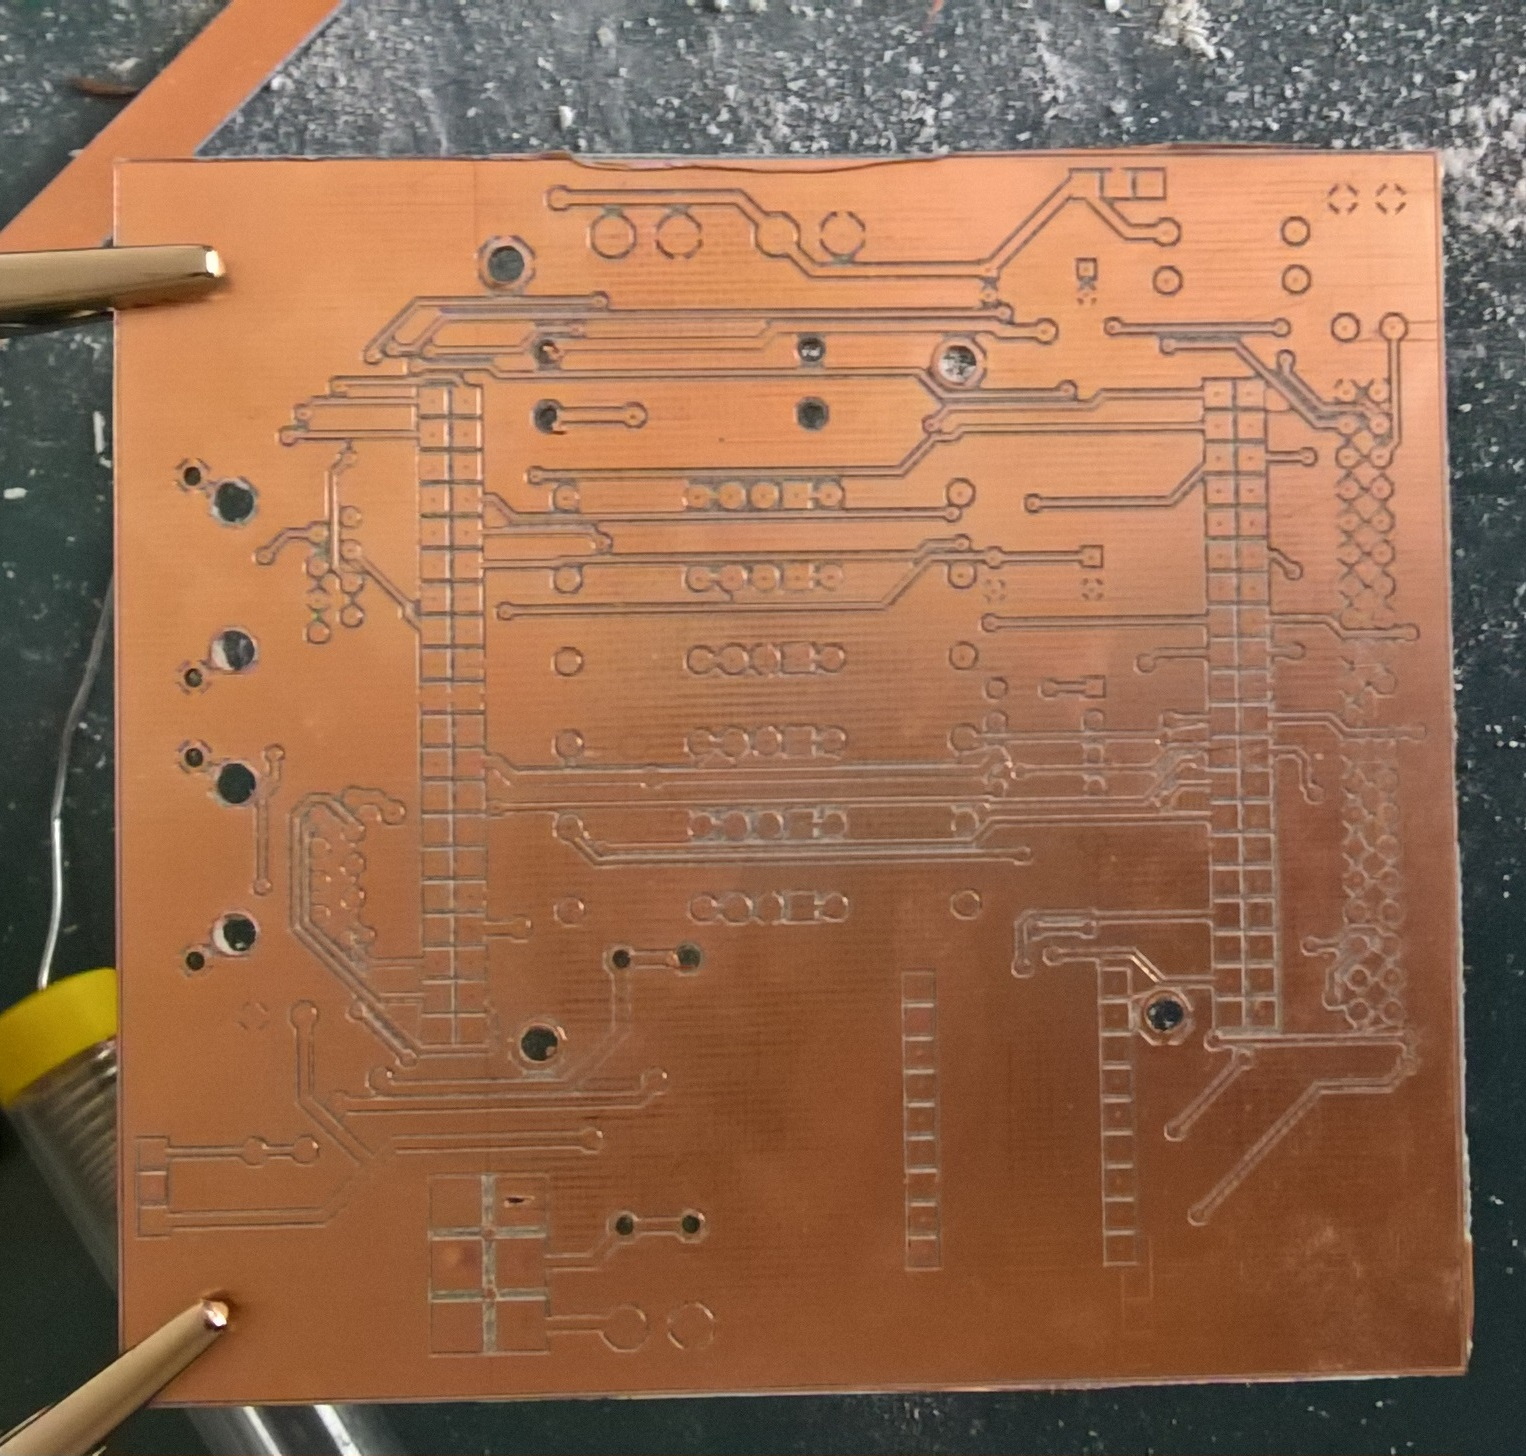
\includegraphics[width=\linewidth]{pictures/main_board_proto.jpg}
        \caption{Прототип}
        \label{fig:main_board_proto}
    \end{subfigure}
    \hfill%
    \begin{subfigure}{0.32\textwidth}
        \centering
        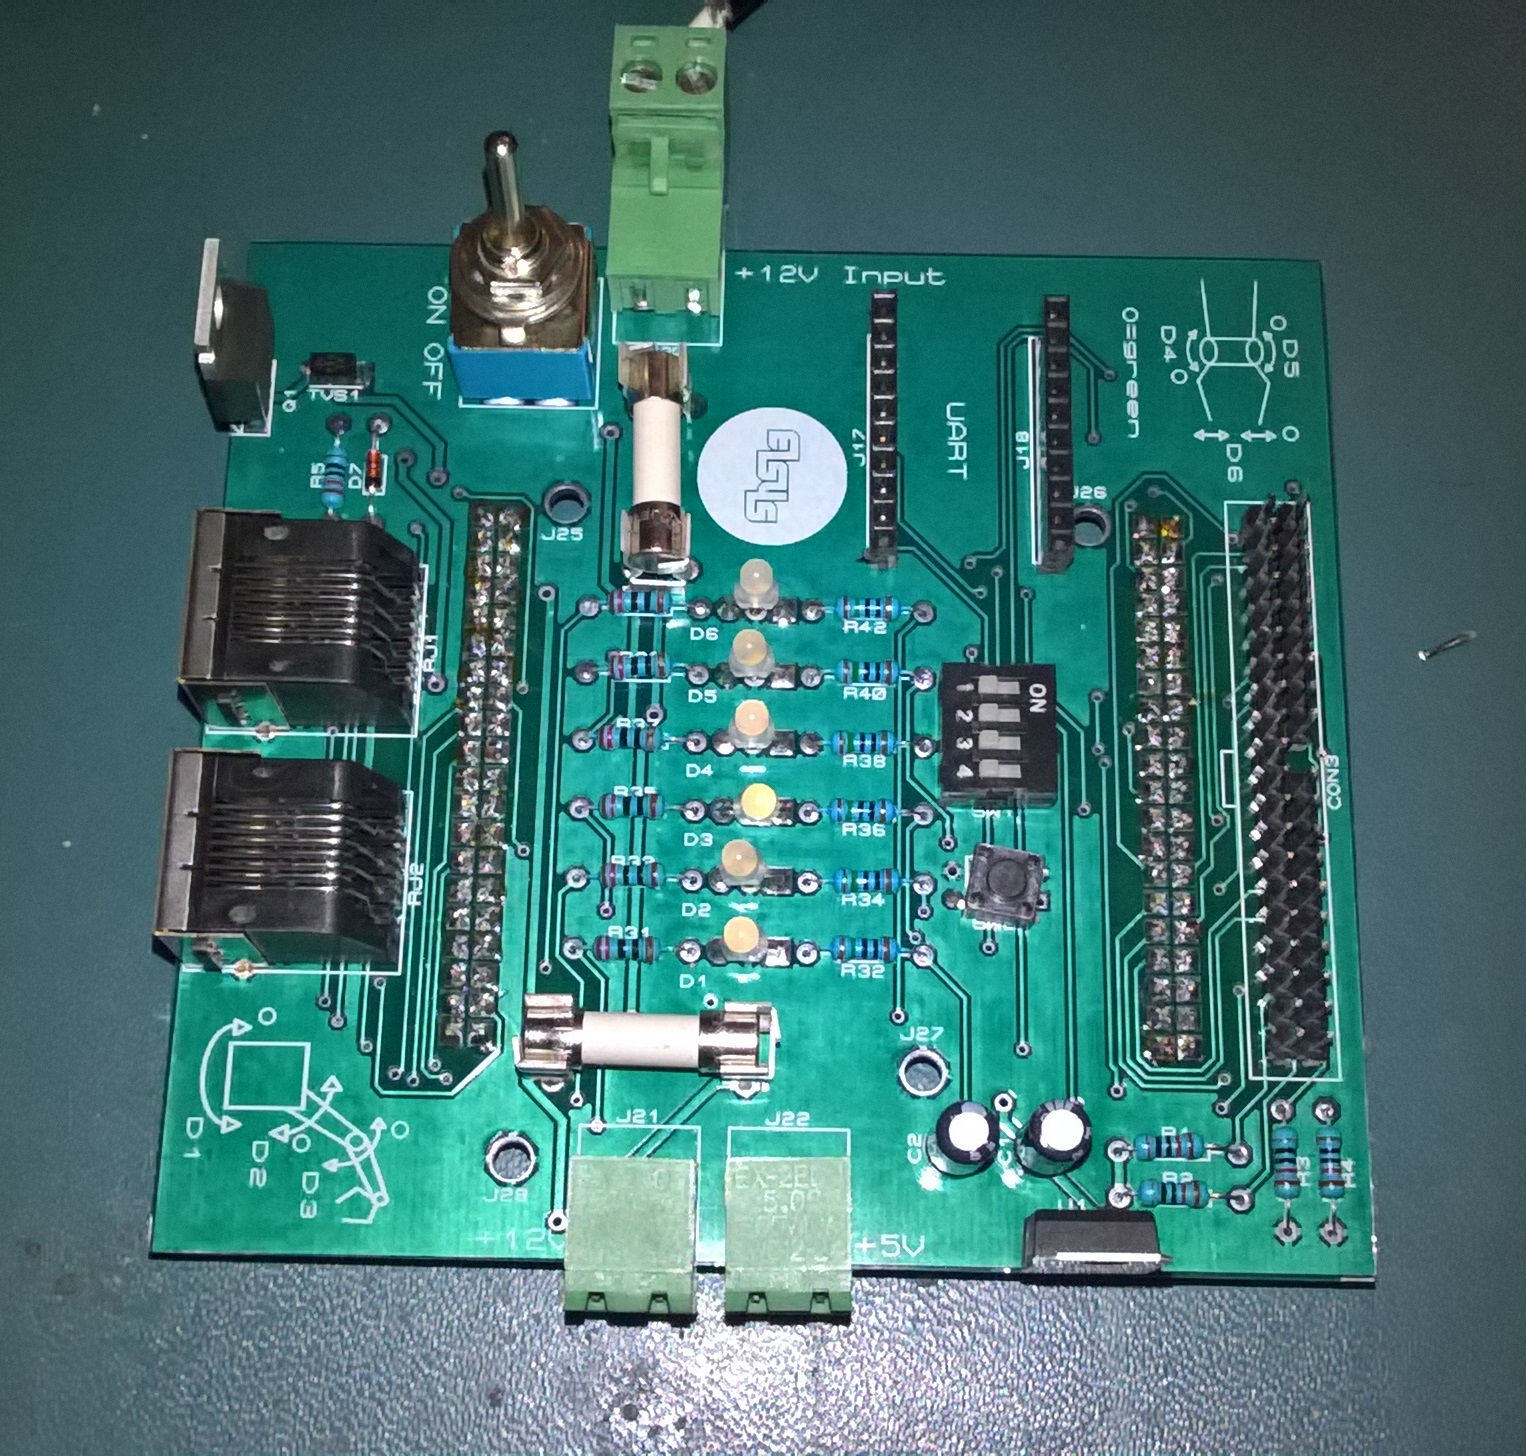
\includegraphics[width=\linewidth]{pictures/main_board.jpg}
        \caption{Завършен вариант}
        \label{fig:main_board_real}
    \end{subfigure}
    \caption{Основна платка}
    \label{fig:main_board}
\end{figure}
\indent{}
На фигура \ref{fig:pcb_sandwich} е показано свързването на готовата основна платка. Микроконтролерната платка се намира под основната. Червено-синият кабел е свързан към захранващия блок, жълто-зеленият кабел е свързан към оптичния сензорен хващач, а светло кафявият - към захранващия порт на РОБКО 01. Зелените кабели са свързани с джойстиците, а сивият лентов кабел с порт B на РОБКО 01. Черният USB кабел се използва за серийна комуникация между сървъра и микроконтролера, а сивият USB кабел за програмиране на микроконтролера.\\
\begin{figure}[!htb]
    \centering
    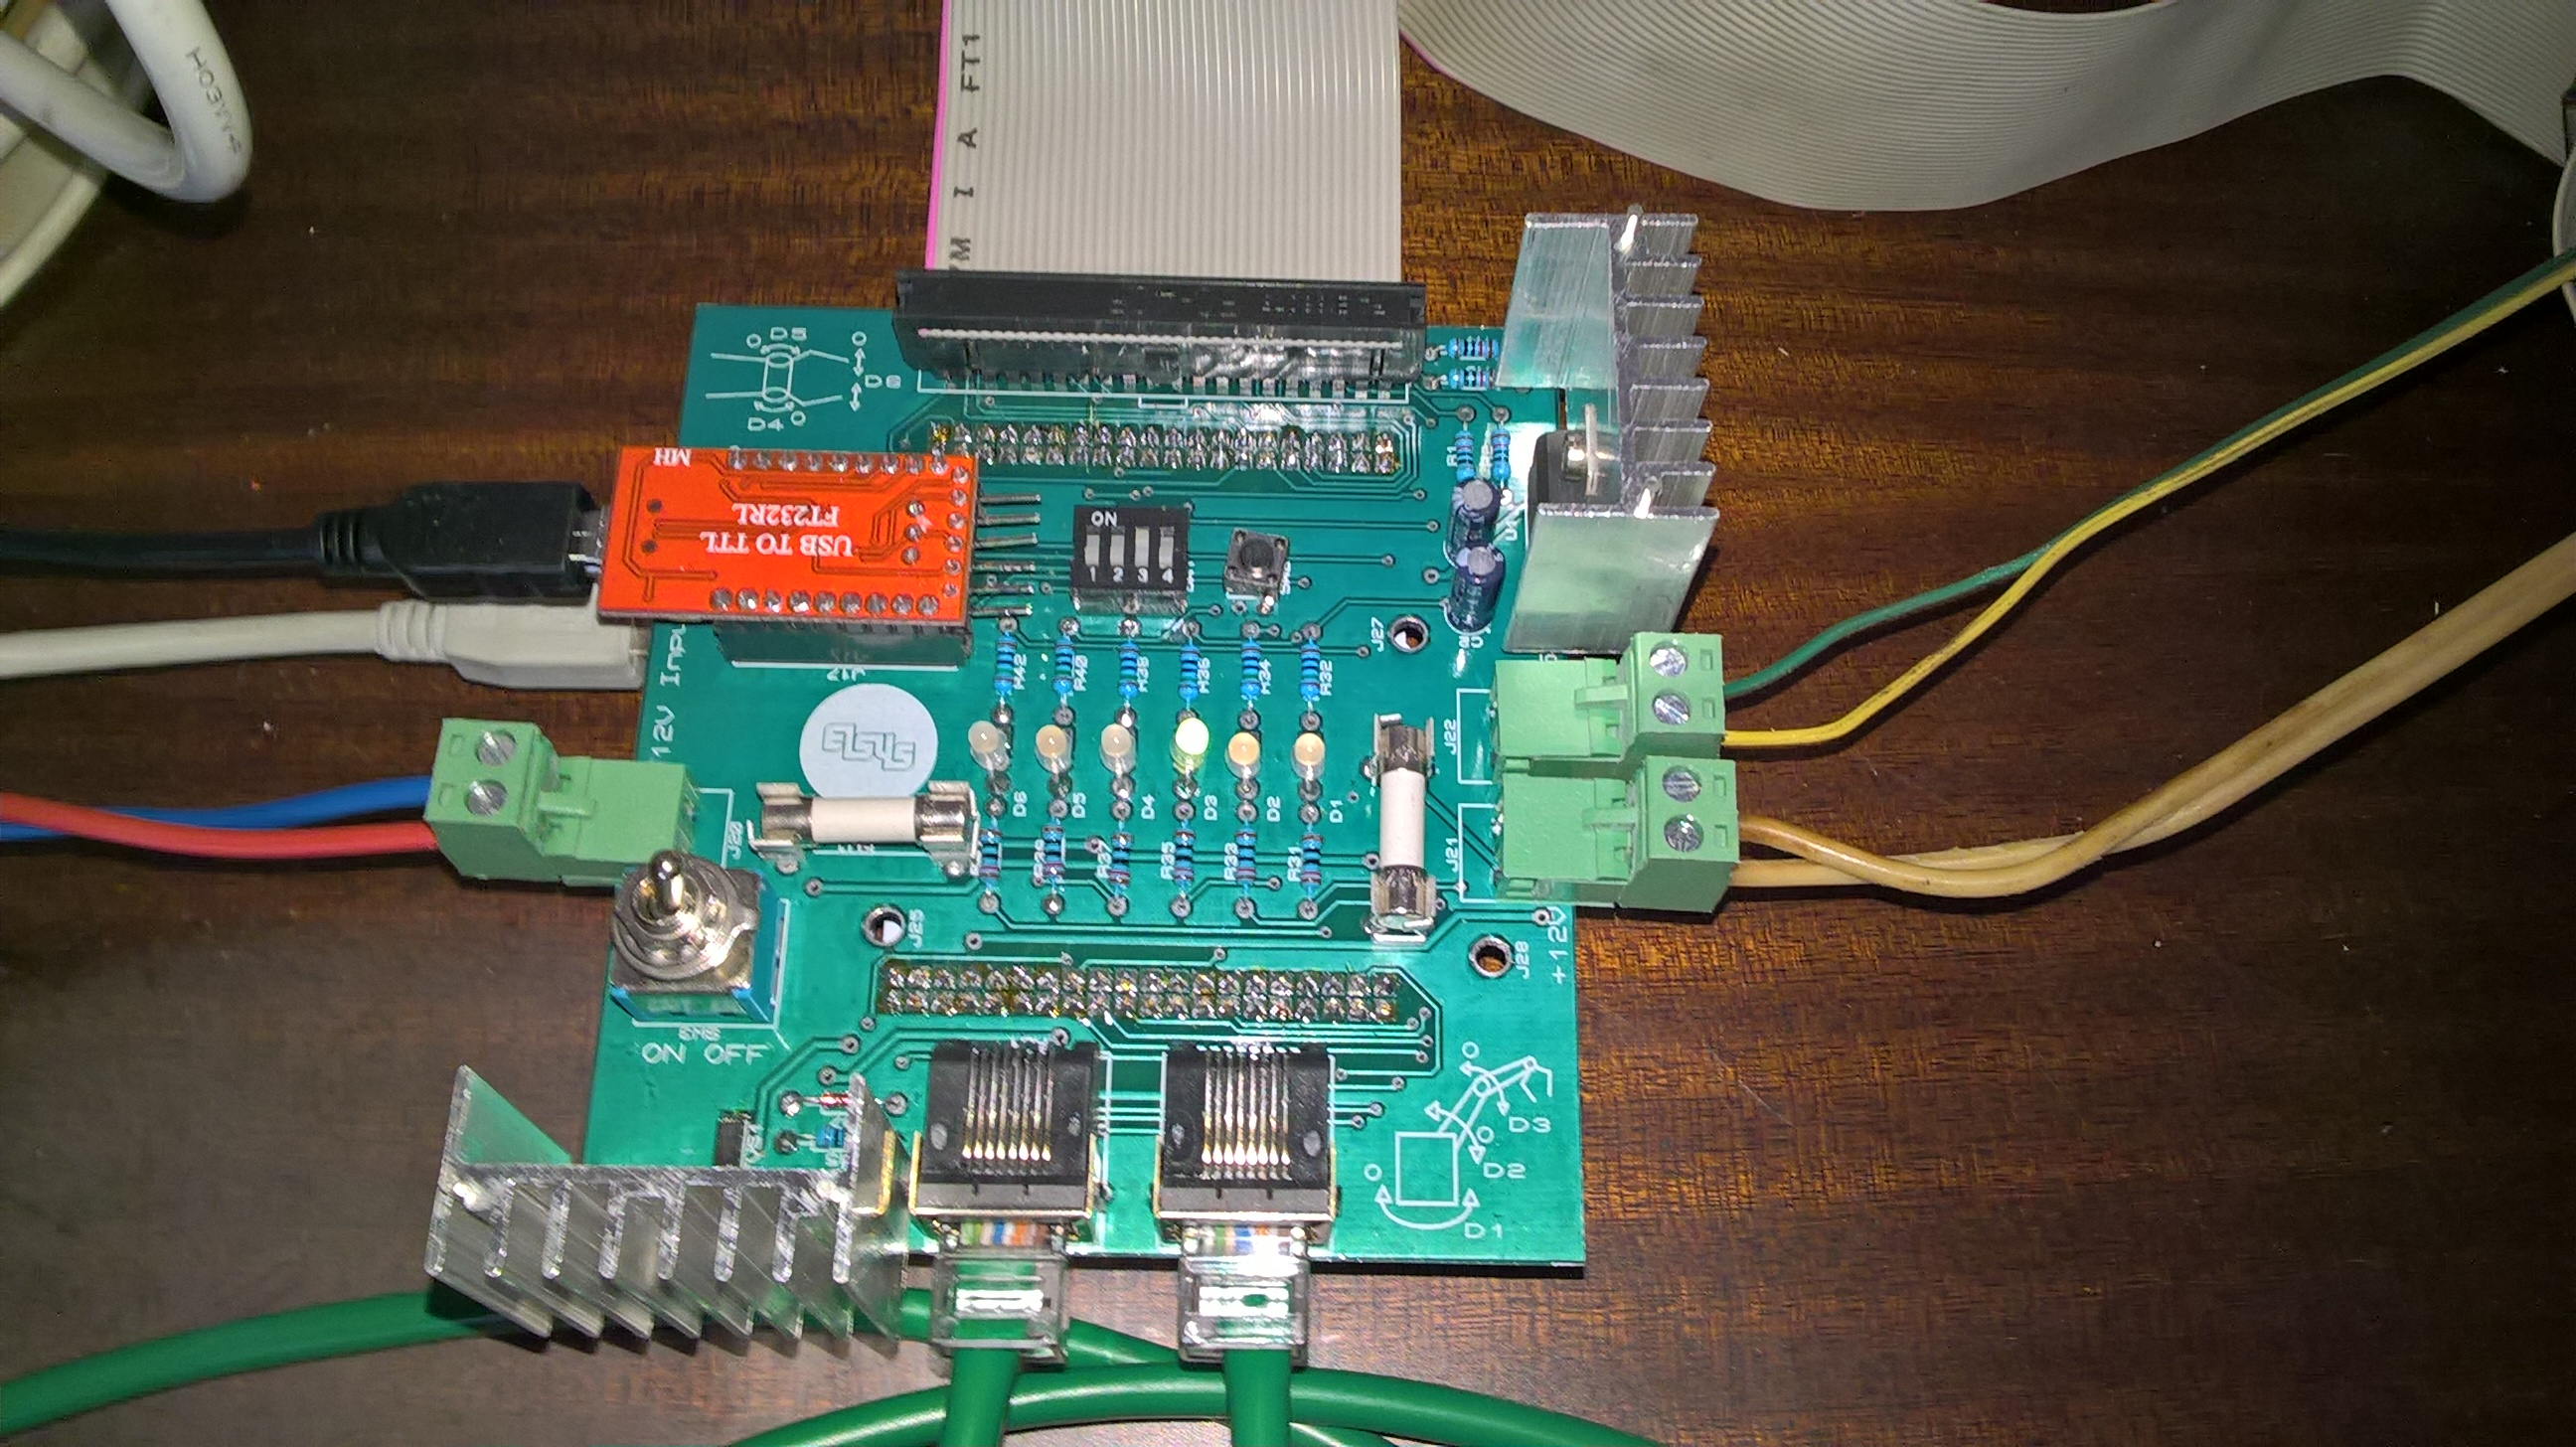
\includegraphics[width=0.8\linewidth]{pictures/all_plugged_in.jpg}
    \captionof{figure}{Основна платка, микроконтролер и USB/UART модул}
    \label{fig:pcb_sandwich}
\end{figure}
\indent{}
На фигура \ref{fig:compl_sys} е показана завършената система.
\begin{figure}[!htb]
    \centering
    %Смени снимката
    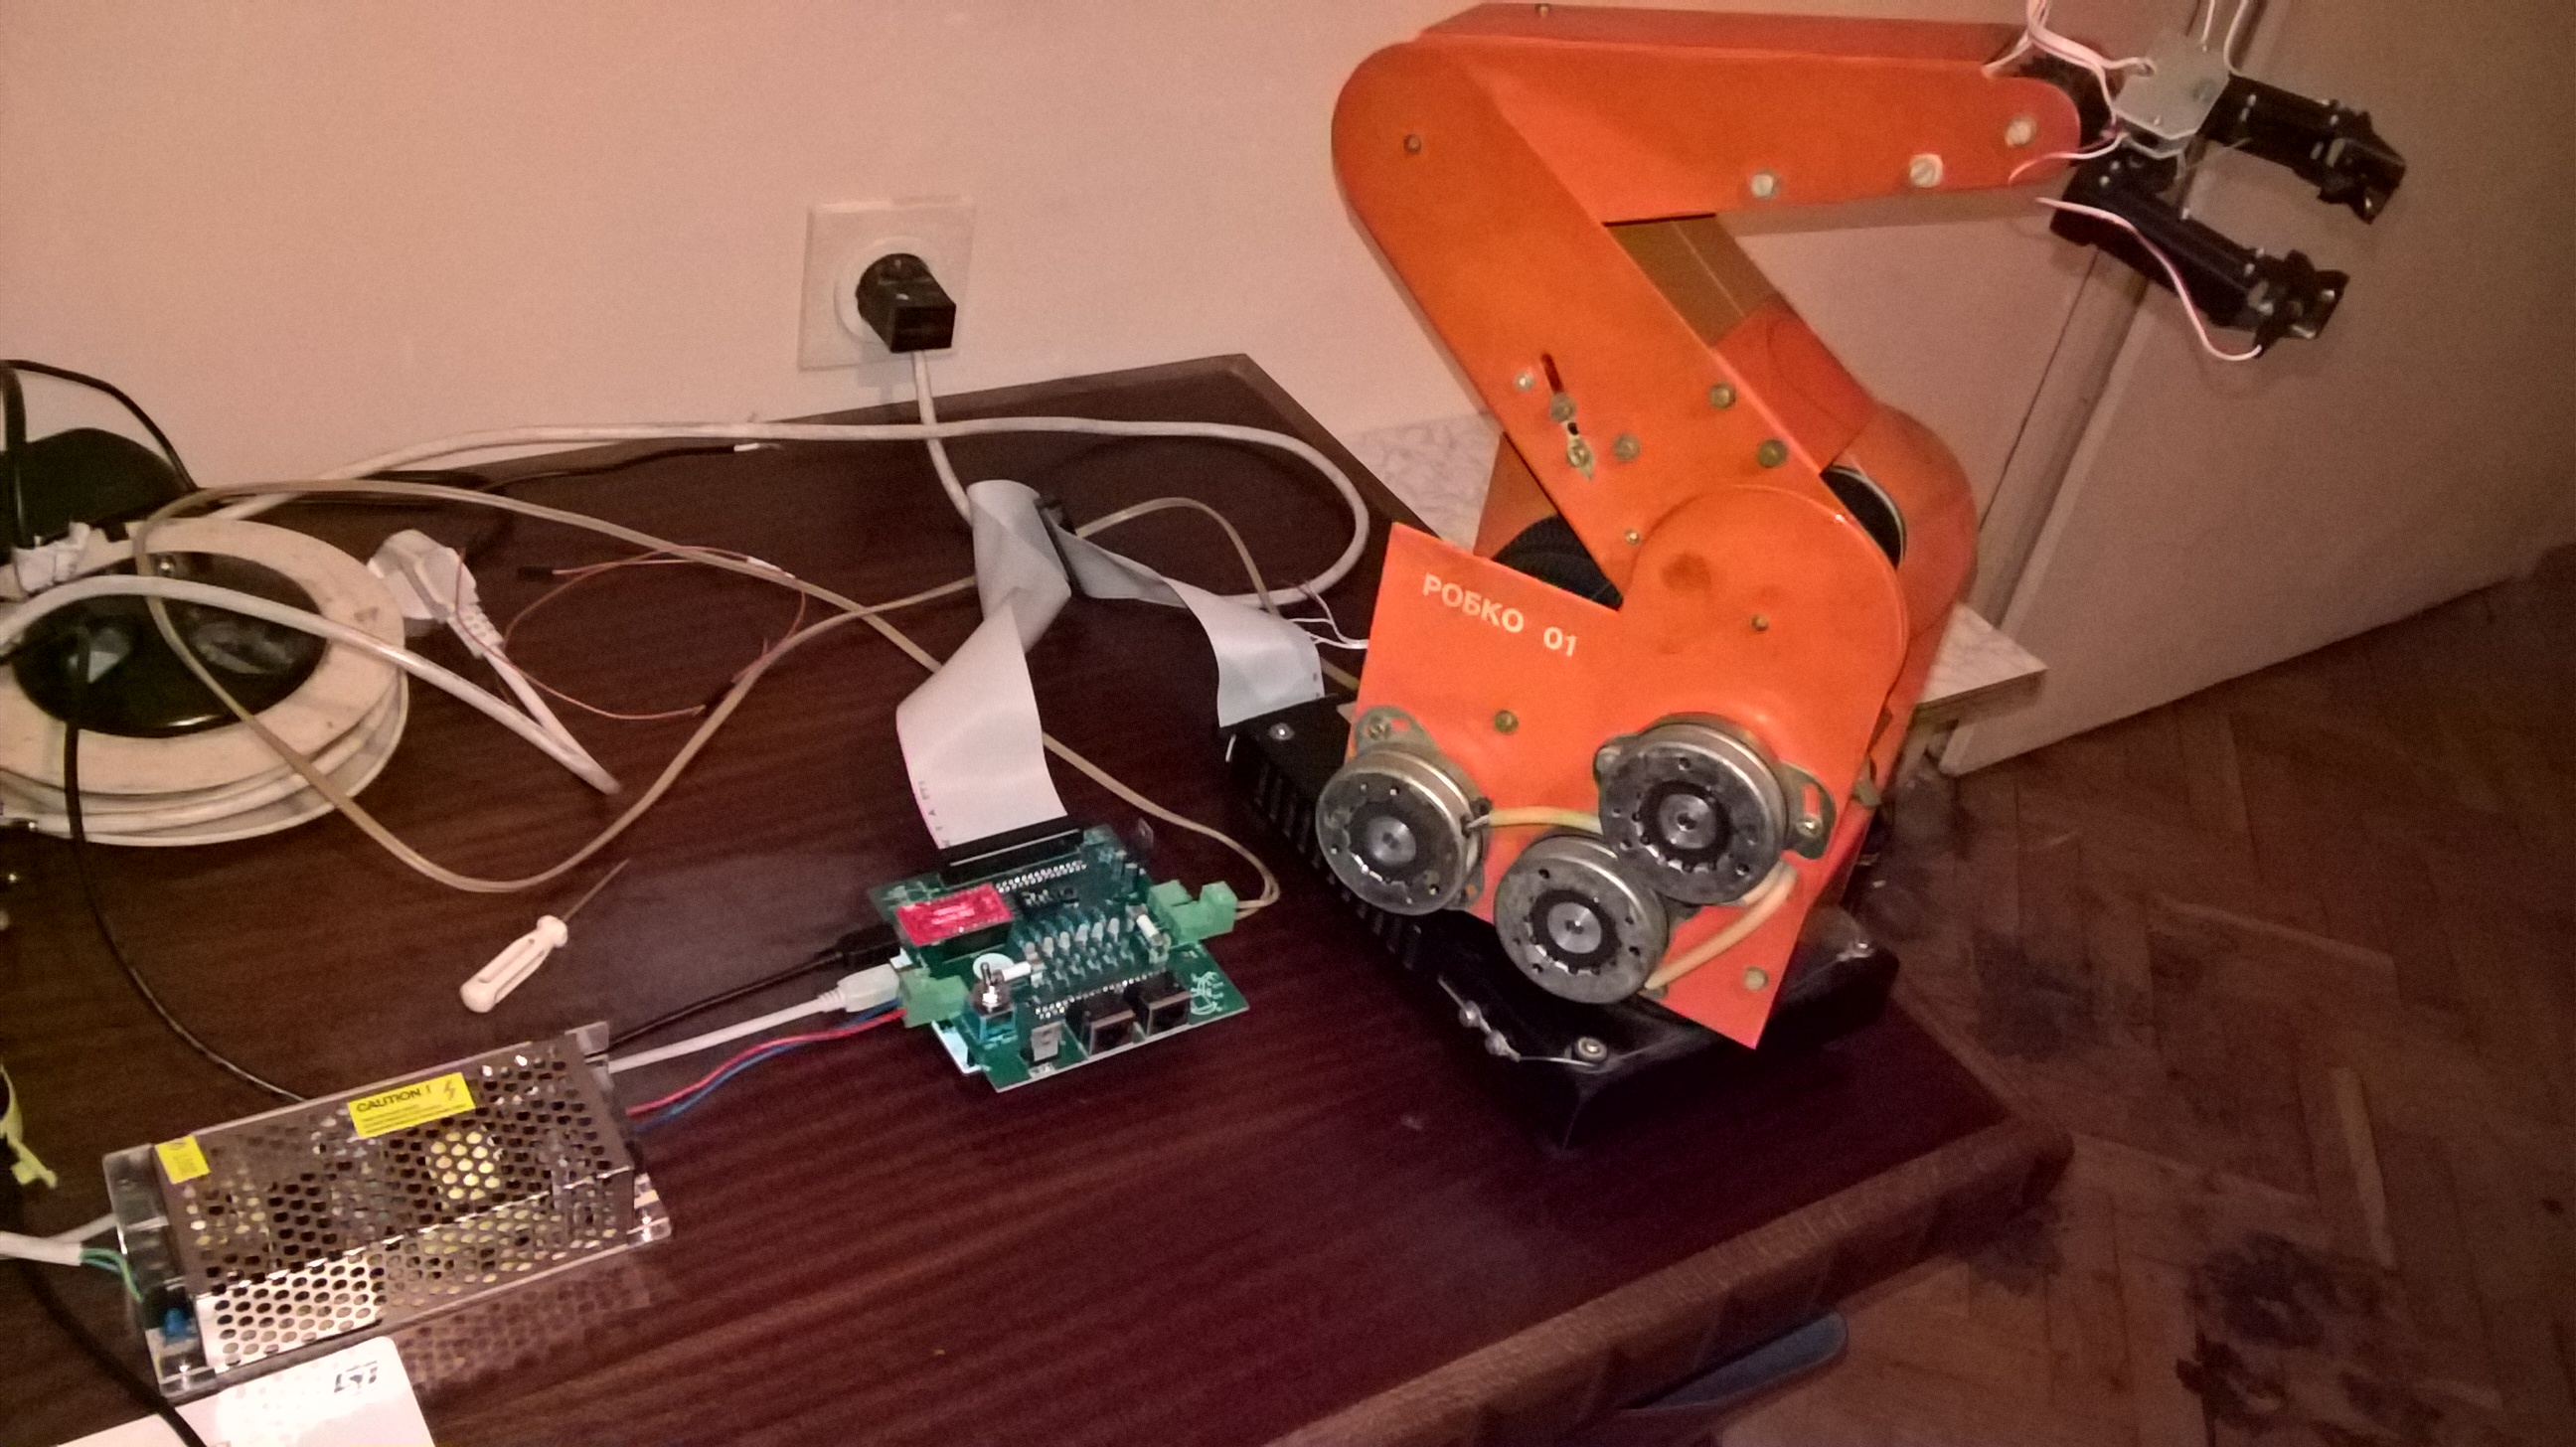
\includegraphics[width=0.8\linewidth]{pictures/completed_system.jpg}
    \captionof{figure}{Завършена система}
    \label{fig:compl_sys}
\end{figure}
